\documentclass[aspectratio=169,11pt]{beamer}

% Theme and colors
\usetheme{Madrid}
\usecolortheme{whale}
\setbeamertemplate{navigation symbols}{}
\setbeamertemplate{footline}[frame number]

% Packages
\usepackage[utf8]{inputenc}
\usepackage[T1]{fontenc}
\usepackage{graphicx}
\usepackage{booktabs}
\usepackage{amsmath}
\usepackage{hyperref}
\usepackage{tikz}
\usetikzlibrary{shapes,arrows,positioning,calc,fit,backgrounds}
\usepackage{siunitx}
\usepackage{xcolor}
\usepackage{array}

% Title information
\title[EECE5155 -- Module 8]{Data Analytics for IoT}
\subtitle{Module 8: From Raw Data to Actionable Intelligence}
\author{Eduardo Baena}
\date{Spring 2026}
\institute{Northeastern University\\Department of Electrical and Computer Engineering\\
\texttt{e.baena@northeastern.edu}}

\begin{document}

%==============================================================================
% SLIDE 1: Title
%==============================================================================
\begin{frame}
    \titlepage
    \begin{center}
        \textbf{EECE5155: Wireless Sensor Networks and the Internet of Things}
    \end{center}
\end{frame}

%==============================================================================
% SLIDE 2: Where are we in the pipeline?
%==============================================================================
\begin{frame}{Where Are We?}
    \begin{center}
    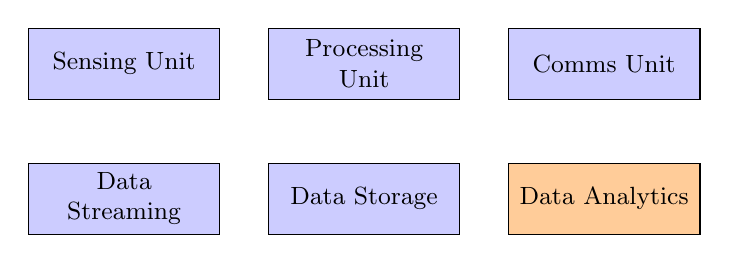
\begin{tikzpicture}[node distance=0.6cm, auto,
        block/.style={rectangle, draw, fill=blue!20, text width=2.2cm, text centered, minimum height=0.9cm, font=\small},
        highlight/.style={rectangle, draw, fill=orange!40, text width=2.2cm, text centered, minimum height=0.9cm, font=\small}]

        \node[block] (sense) {Sensing Unit};
        \node[block, right=of sense] (proc) {Processing Unit};
        \node[block, right=of proc] (comm) {Comms Unit};
        \node[block, below=0.8cm of sense] (stream) {Data Streaming};
        \node[block, below=0.8cm of proc] (storage) {Data Storage};
        \node[highlight, below=0.8cm of comm] (analytics) {Data Analytics};

    \end{tikzpicture}
    \end{center}

    \vspace{0.3cm}
    \begin{itemize}
        \item We know how to \textbf{sense} data (Module 1--2)
        \item We know how to \textbf{stream} it (Module 6) and \textbf{store} it (Module 7)
        \item Now: how do we \textbf{extract value} from all that data?
    \end{itemize}
\end{frame}

%==============================================================================
% SLIDE 3: Outline
%==============================================================================
\begin{frame}{Outline}
    \begin{itemize}
        \item \textbf{Part 1:} Why analytics? The IoT data problem
        \item \textbf{Part 2:} The analytics pipeline
        \item \textbf{Part 3:} Data quality and preprocessing
        \item \textbf{Part 4:} Types of analytics
        \item \textbf{Part 5:} ML overview for IoT (conceptual)
        \item \textbf{Part 6:} Tools, visualization, and delivery
    \end{itemize}
\end{frame}

%==============================================================================
% PART 1: Why analytics?
%==============================================================================

\begin{frame}{The IoT Data Problem}
    \begin{itemize}
        \item \textbf{18.8 billion} connected IoT devices in 2024
        \item \textbf{40 billion} projected by 2030
        \item Most organizations use \textbf{less than 1\%} of their IoT data
        \item The rest sits in cold storage, unanalyzed
    \end{itemize}

    \vspace{0.5cm}
    \begin{alertblock}{Key Insight}
        Raw sensor data has \textbf{no intrinsic value}. The value comes from analysis.
    \end{alertblock}
\end{frame}

\begin{frame}{What Can Analytics Do?}
    \textbf{Real-world impact:}
    \begin{itemize}
        \item \textbf{Predictive maintenance}: 40\% cost reduction in manufacturing
        \item \textbf{Energy optimization}: 20--40\% savings in buildings
        \item \textbf{Quality control}: 95\%+ defect detection in production lines
        \item \textbf{Healthcare}: wearable analytics for early detection
        \item \textbf{Agriculture}: soil monitoring $\rightarrow$ irrigation optimization
    \end{itemize}

    \vspace{0.3cm}
    \begin{block}{The bottleneck is not collection --- it is analysis}
        Sensors are cheap. Making sense of the data is the hard part.
    \end{block}
\end{frame}

\begin{frame}{The Four Vs of IoT Data}
    \begin{itemize}
        \item \textbf{Volume}
        \begin{itemize}
            \item 10k sensors at 1 Hz = 864 million readings per day
        \end{itemize}
        \item \textbf{Velocity}
        \begin{itemize}
            \item Vibration sensors: 10--50 kHz
            \item Temperature: 0.1--1 Hz
            \item Decisions must often match the data rate
        \end{itemize}
        \item \textbf{Variety}
        \begin{itemize}
            \item Floats, integers, JSON, images, audio
            \item Different protocols: MQTT, CoAP, HTTP, OPC-UA
        \end{itemize}
        \item \textbf{Veracity}
        \begin{itemize}
            \item 5--70\% missing data rates in real deployments
            \item Sensor drift, noise, stuck values, duplicates
        \end{itemize}
    \end{itemize}
\end{frame}

%==============================================================================
% PART 2: The analytics pipeline
%==============================================================================

\begin{frame}{The IoT Analytics Pipeline}
    \textbf{Data flows through six stages from sensor to decision:}

    \vspace{0.3cm}
    \begin{center}
    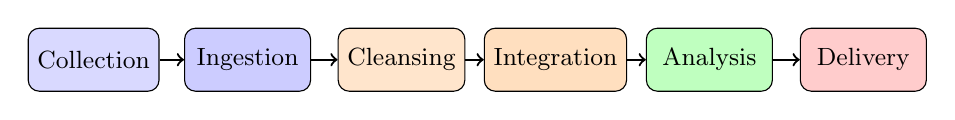
\begin{tikzpicture}[scale=0.85, every node/.style={font=\small}]
        \node[draw, fill=blue!15, minimum width=1.6cm, minimum height=0.8cm, rounded corners] (col) at (0,0) {Collection};
        \node[draw, fill=blue!20, minimum width=1.6cm, minimum height=0.8cm, rounded corners] (ing) at (2.3,0) {Ingestion};
        \node[draw, fill=orange!20, minimum width=1.6cm, minimum height=0.8cm, rounded corners] (cln) at (4.6,0) {Cleansing};
        \node[draw, fill=orange!25, minimum width=1.6cm, minimum height=0.8cm, rounded corners] (int) at (6.9,0) {Integration};
        \node[draw, fill=green!25, minimum width=1.6cm, minimum height=0.8cm, rounded corners] (ana) at (9.2,0) {Analysis};
        \node[draw, fill=red!20, minimum width=1.6cm, minimum height=0.8cm, rounded corners] (del) at (11.5,0) {Delivery};

        \draw[->, thick] (col) -- (ing);
        \draw[->, thick] (ing) -- (cln);
        \draw[->, thick] (cln) -- (int);
        \draw[->, thick] (int) -- (ana);
        \draw[->, thick] (ana) -- (del);
    \end{tikzpicture}
    \end{center}

    \vspace{0.3cm}
    \begin{block}{}
        This is the same pipeline regardless of your application domain. The tools and algorithms change, but the stages do not.
    \end{block}
\end{frame}

\begin{frame}{Stage 1: Collection}
    \textbf{Getting data from sensors to a central point}
    \begin{itemize}
        \item Multiple sensor types, different firmware versions
        \item Mixed protocols: MQTT, CoAP, HTTP, OPC-UA
        \item Bursty traffic: 10k devices reconnect simultaneously after power outage
        \item Clock drift and timezone mismatches
    \end{itemize}

    \vspace{0.3cm}
    \textbf{You already know how to do this:}
    \begin{itemize}
        \item Module 6: MQTT, CoAP (streaming protocols)
        \item Module 7: InfluxDB, Parquet (storage)
    \end{itemize}
\end{frame}

\begin{frame}{Stage 2: Ingestion}
    \textbf{Getting all data into a single data store at scale}
    \begin{itemize}
        \item \textbf{Batch}: load periodically (e.g., hourly ETL job)
        \item \textbf{Micro-batch}: process every few seconds (Spark Streaming)
        \item \textbf{Stream}: process as it arrives, millisecond latency (Flink, Kafka)
    \end{itemize}

    \vspace{0.5cm}
    \begin{alertblock}{Design Principle}
        Ingest first, validate later. Synchronous validation at broker scale is a bottleneck. Validate downstream.
    \end{alertblock}
\end{frame}

\begin{frame}{Stages 3--4: Cleansing and Integration}
    \textbf{Cleansing: fix the data}
    \begin{itemize}
        \item Remove duplicates (MQTT QoS 1 can cause them)
        \item Handle missing values (forward-fill, interpolation)
        \item Detect and flag outliers
        \item Normalize formats and units
    \end{itemize}

    \vspace{0.3cm}
    \textbf{Integration: combine the data}
    \begin{itemize}
        \item Join sensor data with metadata (device ID $\rightarrow$ location, type)
        \item Enrich with external data (weather, schedules)
        \item Resolve timestamp conflicts across devices
    \end{itemize}
\end{frame}

\begin{frame}{Stages 5--6: Analysis and Delivery}
    \textbf{Analysis: extract intelligence}
    \begin{itemize}
        \item Statistics, rules, machine learning
        \item This is the core of this module --- more detail coming
    \end{itemize}

    \vspace{0.3cm}
    \textbf{Delivery: get insights to decision-makers}
    \begin{itemize}
        \item Dashboards (Grafana, Kibana, Power BI)
        \item Alerts (email, Slack, PagerDuty)
        \item APIs (REST endpoints for other systems)
        \item Reports (automated PDF, email digest)
    \end{itemize}

    \vspace{0.3cm}
    \begin{block}{Remember}
        Analytics value is realized \textbf{only} when insights reach the right person at the right time.
    \end{block}
\end{frame}

%==============================================================================
% PART 3: Data quality
%==============================================================================

\begin{frame}{Data Quality: The Hidden Problem}
    \begin{center}
        \Large
        \textbf{Real IoT data is messy}
    \end{center}

    \vspace{0.5cm}
    \textbf{A systematic review of 57 IoT publications found 8 common error types.}

    \vspace{0.3cm}
    Next slide: let's look at each one.
\end{frame}

\begin{frame}{The 8 Sensor Error Types}
    \begin{center}
    \begin{tabular}{lll}
        \toprule
        \textbf{Error Type} & \textbf{Frequency} & \textbf{Example} \\
        \midrule
        Outliers & Most common & Spike: 200\textdegree C from a 25\textdegree C sensor \\
        Missing data & Very common & 5--70\% missing in real deployments \\
        Bias / offset & Common & Sensor reads 2\textdegree C too high \\
        Drift & Common & Gradual deviation over months \\
        Noise & Common & Random fluctuation around true value \\
        Constant / stuck & Moderate & Sensor locked at last value \\
        Uncertainty & Moderate & Calibration tolerance not modeled \\
        Stuck-at-zero & Less common & Reset condition or division-by-zero \\
        \bottomrule
    \end{tabular}
    \end{center}
\end{frame}

\begin{frame}{Which Errors Can You Fix?}
    \begin{itemize}
        \item \textbf{Outliers}: detectable with $\mu \pm 3\sigma$ or IQR per device
        \item \textbf{Missing data}: fill with last known value (forward-fill) or interpolate
        \item \textbf{Noise}: filter with moving average or Kalman filter
        \item \textbf{Duplicates}: deduplicate by device ID + timestamp
        \item \textbf{Stuck sensor}: detect if last N readings are identical
    \end{itemize}

    \vspace{0.3cm}
    \begin{alertblock}{Drift is the hardest}
        Unlike noise (filterable) or outliers (detectable), drift is a gradual, permanent deviation. It requires recalibration or ML-based correction.
    \end{alertblock}
\end{frame}

\begin{frame}{The Preprocessing Pipeline}
    \textbf{Standard sequence for IoT sensor data:}

    \vspace{0.3cm}
    \begin{center}
    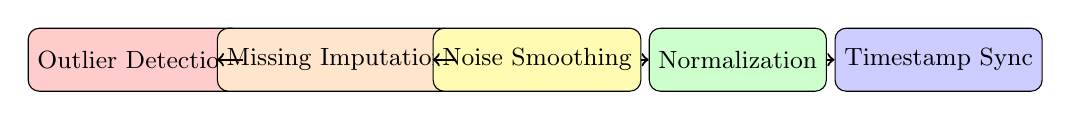
\begin{tikzpicture}[scale=0.85, every node/.style={font=\small}]
        \node[draw, fill=red!20, minimum width=1.6cm, minimum height=0.8cm, rounded corners] (n0) at (0,0) {Outlier Detection};
        \node[draw, fill=orange!20, minimum width=1.6cm, minimum height=0.8cm, rounded corners] (n1) at (3,0) {Missing Imputation};
        \node[draw, fill=yellow!30, minimum width=1.6cm, minimum height=0.8cm, rounded corners] (n2) at (6,0) {Noise Smoothing};
        \node[draw, fill=green!20, minimum width=1.6cm, minimum height=0.8cm, rounded corners] (n3) at (9,0) {Normalization};
        \node[draw, fill=blue!20, minimum width=1.6cm, minimum height=0.8cm, rounded corners] (n4) at (12,0) {Timestamp Sync};
        \draw[->, thick] (n0) -- (n1);
        \draw[->, thick] (n1) -- (n2);
        \draw[->, thick] (n2) -- (n3);
        \draw[->, thick] (n3) -- (n4);
    \end{tikzpicture}
    \end{center}

    \vspace{0.3cm}
    \begin{block}{Key Rule}
        Do not impute flagged outliers. Mark them, exclude them, then impute the gap.
    \end{block}
\end{frame}

%==============================================================================
% PART 4: Types of analytics
%==============================================================================

\begin{frame}{Four Types of Analytics}
    \textbf{Increasing value, increasing complexity:}

    \vspace{0.3cm}
    \begin{center}
    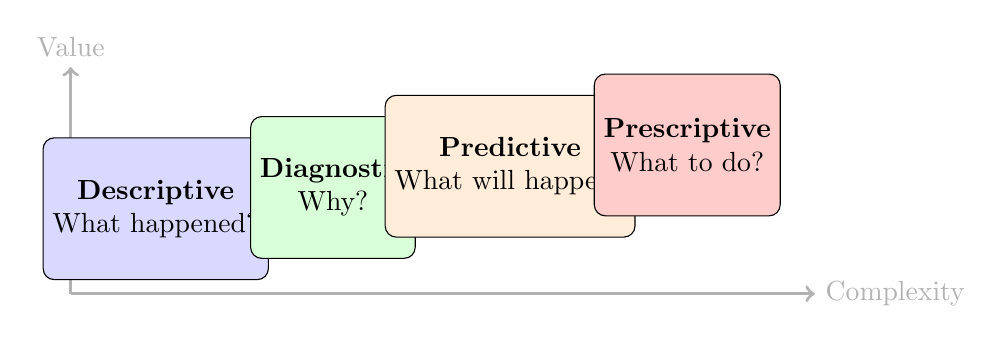
\begin{tikzpicture}[scale=0.9]
        \draw[->, very thick, gray!60] (0,0) -- (10.5,0) node[right] {Complexity};
        \draw[->, very thick, gray!60] (0,0) -- (0,3.2) node[above] {Value};

        \node[draw, fill=blue!15, minimum width=2cm, minimum height=1.8cm, rounded corners, align=center] at (1.2,1.2) {\textbf{Descriptive}\\What happened?};
        \node[draw, fill=green!15, minimum width=2cm, minimum height=1.8cm, rounded corners, align=center] at (3.7,1.5) {\textbf{Diagnostic}\\Why?};
        \node[draw, fill=orange!15, minimum width=2cm, minimum height=1.8cm, rounded corners, align=center] at (6.2,1.8) {\textbf{Predictive}\\What will happen?};
        \node[draw, fill=red!20, minimum width=2cm, minimum height=1.8cm, rounded corners, align=center] at (8.7,2.1) {\textbf{Prescriptive}\\What to do?};
    \end{tikzpicture}
    \end{center}
\end{frame}

\begin{frame}{Descriptive Analytics}
    \textbf{``What happened?''}
    \begin{itemize}
        \item Dashboards showing current and historical sensor readings
        \item KPIs: average temperature, uptime percentage, packet loss rate
        \item Aggregations: hourly/daily/weekly summaries
        \item Data exploration: distributions, correlations, trends
    \end{itemize}

    \vspace{0.3cm}
    \textbf{Tools:} Grafana, Kibana, Power BI, DuckDB queries

    \vspace{0.3cm}
    \begin{exampleblock}{This is where most IoT deployments are today}
        Descriptive analytics is the foundation. If you can't describe your data, you can't analyze it.
    \end{exampleblock}
\end{frame}

\begin{frame}{Diagnostic Analytics}
    \textbf{``Why did it happen?''}
    \begin{itemize}
        \item Root-cause analysis: drill down from KPI anomaly to specific sensor
        \item Correlation: which sensors are correlated with failures?
        \item Comparison: this week vs. last week, zone A vs. zone B
        \item Example: temperature spike $\rightarrow$ HVAC failure $\rightarrow$ clogged filter
    \end{itemize}

    \vspace{0.3cm}
    \textbf{Tools:} SQL queries, Grafana drill-down, pandas/DuckDB

    \vspace{0.3cm}
    \begin{block}{}
        Often done manually by engineers. The goal is to automate the investigation.
    \end{block}
\end{frame}

\begin{frame}{Predictive Analytics}
    \textbf{``What will happen?''}
    \begin{itemize}
        \item Machine learning models trained on historical data
        \item Predict: when will this machine fail? (Remaining Useful Life)
        \item Forecast: what will energy consumption be tomorrow?
        \item Classify: is this reading normal or anomalous?
    \end{itemize}

    \vspace{0.3cm}
    \textbf{This requires ML --- but not always deep learning.}
    \begin{itemize}
        \item Many IoT problems are solved with simple models (thresholds, regression)
        \item Deep learning only when simpler approaches fail
    \end{itemize}
\end{frame}

\begin{frame}{Prescriptive Analytics}
    \textbf{``What should we do?''}
    \begin{itemize}
        \item Optimization: adjust HVAC setpoints to minimize energy
        \item Closed-loop control: sensor $\rightarrow$ model $\rightarrow$ actuator
        \item Recommendations: ``Replace bearing in machine 3 within 5 days''
        \item Scheduling: plan maintenance during low-production windows
    \end{itemize}

    \vspace{0.3cm}
    \begin{alertblock}{The Holy Grail}
        Very few IoT deployments reach prescriptive analytics. It requires trust in the models, closed-loop infrastructure, and organizational buy-in.
    \end{alertblock}
\end{frame}

%==============================================================================
% PART 5: ML overview
%==============================================================================

\begin{frame}{Machine Learning: A Quick Overview}
    \begin{center}
        \Large
        \textbf{What is a Machine Learning model?}
    \end{center}

    \vspace{0.5cm}
    \begin{itemize}
        \item A mathematical function that maps inputs to outputs
        \item \textbf{Learned automatically} from data, not programmed by hand
        \item You already know the simplest one: linear regression ($y = mx + b$)
        \item ML generalizes this to any function, any number of inputs
    \end{itemize}
\end{frame}

\begin{frame}{ML in IoT Terms}
    \begin{itemize}
        \item \textbf{Input}: sensor readings (temperature, vibration, current\ldots)
        \item \textbf{Output}: a decision
        \begin{itemize}
            \item ``This bearing has fault type A'' (classification)
            \item ``Remaining useful life = 12 days'' (regression)
            \item ``This reading is anomalous'' (anomaly detection)
        \end{itemize}
        \item \textbf{Training}: finding the best function using historical labeled data
        \item \textbf{Inference}: applying that function to new, unseen data
    \end{itemize}

    \vspace{0.3cm}
    \begin{block}{Intuition}
        Training = automated curve fitting on historical data. Inference = using that curve on live data.
    \end{block}
\end{frame}

\begin{frame}{Three Problem Types}
    \begin{columns}[T]
        \begin{column}{0.32\textwidth}
            \textbf{Classification}
            \begin{itemize}
                \item Assign a label
                \item ``Normal'' vs ``Fault A'' vs ``Fault B''
                \item Algorithms: Random Forest, XGBoost
            \end{itemize}
        \end{column}
        \begin{column}{0.32\textwidth}
            \textbf{Regression}
            \begin{itemize}
                \item Predict a number
                \item ``RUL = 12 days''
                \item Algorithms: Linear Regression, LSTM
            \end{itemize}
        \end{column}
        \begin{column}{0.32\textwidth}
            \textbf{Anomaly Detection}
            \begin{itemize}
                \item Flag unusual patterns
                \item No labels needed
                \item Algorithms: Autoencoder, Isolation Forest
            \end{itemize}
        \end{column}
    \end{columns}
\end{frame}

\begin{frame}{Overfitting: The Main Trap}
    \textbf{How do we know if a model is good --- or just memorizing?}

    \vspace{0.3cm}
    \begin{itemize}
        \item Split your data into \textbf{training} (70\%), \textbf{validation} (15\%), \textbf{test} (15\%)
        \item Train on training set, tune on validation, evaluate honestly on test
        \item \textbf{Overfitting}: model memorizes training noise, fails on new data
        \item \textbf{Underfitting}: model too simple, misses real patterns
    \end{itemize}

    \vspace{0.3cm}
    \begin{alertblock}{IoT-Specific Warning}
        Time-series data is \textbf{not} random. Never shuffle! Use \textbf{walk-forward validation}: train on past, test on future. Otherwise the model ``cheats'' by seeing the future.
    \end{alertblock}
\end{frame}

\begin{frame}{Algorithm Selection: Keep It Simple}
    \textbf{Practical rule for IoT:}

    \vspace{0.3cm}
    \begin{center}
    \begin{tabular}{lll}
        \toprule
        \textbf{Problem} & \textbf{Start with} & \textbf{If not enough} \\
        \midrule
        Classification & Random Forest / XGBoost & CNN or LSTM \\
        Regression (RUL) & Linear Regression & LSTM \\
        Anomaly detection & Threshold rules & Autoencoder \\
        Forecasting & Moving average & Prophet / Chronos \\
        \bottomrule
    \end{tabular}
    \end{center}

    \vspace{0.3cm}
    \begin{exampleblock}{Start simple}
        XGBoost on engineered features beats deep learning on most IoT tabular datasets with less than 10k labeled samples.
    \end{exampleblock}
\end{frame}

\begin{frame}{Feature Engineering: Why It Matters}
    \textbf{Raw sensor values are rarely the right input to a model.}

    \vspace{0.3cm}
    \begin{itemize}
        \item Instead of feeding 1000 raw temperature readings, compute:
        \begin{itemize}
            \item Mean, standard deviation, min, max
            \item Rate of change
            \item Percentiles (P5, P95)
            \item Zero-crossing rate
        \end{itemize}
        \item These are called \textbf{features}
        \item Compute features over a \textbf{window} of time (e.g., last 5 minutes)
    \end{itemize}

    \vspace{0.3cm}
    \begin{block}{The Window}
        \textbf{Tumbling}: non-overlapping (each sample used once)\\
        \textbf{Sliding}: overlapping (richer context, more computation)\\
        \textbf{Session}: event-triggered (variable length)
    \end{block}
\end{frame}

%==============================================================================
% PART 6: Tools and visualization
%==============================================================================

\begin{frame}{Stream Analytics: Real-Time Intelligence}
    \textbf{Sometimes you cannot wait for batch processing.}

    \vspace{0.3cm}
    \begin{itemize}
        \item \textbf{Apache Flink}: true streaming, sub-100 ms latency
        \item \textbf{Spark Structured Streaming}: micro-batch, 100 ms--1 s
        \item \textbf{Kafka Streams}: SQL-like queries embedded in Kafka
    \end{itemize}

    \vspace{0.3cm}
    \textbf{When to use stream vs batch:}
    \begin{itemize}
        \item Real-time alerts (temperature exceeds threshold) $\rightarrow$ \textbf{stream}
        \item Daily energy report $\rightarrow$ \textbf{batch}
        \item Anomaly detection on live data $\rightarrow$ \textbf{stream}
        \item Training an ML model $\rightarrow$ \textbf{batch}
    \end{itemize}
\end{frame}

\begin{frame}{Analytics Tools (2026)}
    \begin{center}
    \begin{tabular}{llll}
        \toprule
        \textbf{Tool} & \textbf{Best for} & \textbf{Mode} & \textbf{License} \\
        \midrule
        Apache Spark & Large-scale ETL + ML & Batch + micro-batch & Open source \\
        Apache Flink & Real-time streaming & Stream & Open source \\
        Databricks & Full pipeline & All & Commercial \\
        DuckDB & Ad-hoc queries on Parquet & Batch & Open source \\
        InfluxDB & Time-series queries & Real-time & Open source \\
        \bottomrule
    \end{tabular}
    \end{center}

    \vspace{0.3cm}
    \begin{exampleblock}{DuckDB for IoT analytics}
        Query years of Parquet files directly from a Python notebook. No cluster, no ETL, no cost beyond S3 storage. Ideal for exploratory analytics on cold data.
    \end{exampleblock}
\end{frame}

\begin{frame}{Visualization and Dashboards}
    \textbf{Analytics is useless if nobody sees the results.}

    \vspace{0.3cm}
    \begin{itemize}
        \item \textbf{Grafana}: open-source, connects to InfluxDB/Prometheus
        \begin{itemize}
            \item Time-series graphs, gauges, heatmaps, alerts
            \item The most deployed IoT dashboard stack
        \end{itemize}
        \item \textbf{Kibana}: log and event analytics (OpenSearch/Elasticsearch)
        \item \textbf{Power BI / Tableau}: business intelligence, executive reports
    \end{itemize}

    \vspace{0.3cm}
    \textbf{Alerting:}
    \begin{itemize}
        \item Grafana threshold alerts: ``notify if temp $>$ 30\textdegree C for 5 min''
        \item Use hysteresis to avoid flapping (fires at 30, clears at 28)
    \end{itemize}
\end{frame}

\begin{frame}{Predictive Maintenance: The Flagship Application}
    \textbf{Predict equipment failure before it happens.}

    \vspace{0.3cm}
    \begin{itemize}
        \item Sensors: vibration, temperature, current, pressure
        \item Pipeline: MQTT $\rightarrow$ Kafka $\rightarrow$ feature extraction $\rightarrow$ ML model
        \item Output: Remaining Useful Life (RUL) in days or cycles
    \end{itemize}

    \vspace{0.3cm}
    \textbf{Real impact:}
    \begin{itemize}
        \item 40\% maintenance cost reduction
        \item 50\% less unplanned downtime
    \end{itemize}

    \vspace{0.3cm}
    \textbf{Benchmark datasets (for your project or future research):}
    \begin{itemize}
        \item \textbf{NASA C-MAPSS}: turbofan degradation, 21 sensors, 1000+ papers
        \item \textbf{CWRU Bearing}: vibration data, de facto standard
    \end{itemize}
\end{frame}

\begin{frame}{Emerging: Foundation Models for Time-Series}
    \textbf{Biggest recent shift (2025--2026): pre-trained models that work zero-shot.}

    \vspace{0.3cm}
    \begin{itemize}
        \item \textbf{Problem}: labeling IoT data is expensive and slow
        \item \textbf{Solution}: foundation models trained on millions of time-series
        \item \textbf{Chronos} (Amazon): zero-shot matches fine-tuned models on 42 datasets
        \item \textbf{TimesFM} (Google): 16$\times$ faster than fine-tuning
    \end{itemize}

    \vspace{0.3cm}
    \begin{alertblock}{Practical Guidance}
        No labels? $\rightarrow$ Try Chronos/TimesFM zero-shot.\\
        Some labels? $\rightarrow$ Fine-tune a foundation model.\\
        Anomaly only? $\rightarrow$ Autoencoder on normal data.
    \end{alertblock}
\end{frame}

\begin{frame}{Digital Twins}
    \textbf{A digital twin = virtual model synchronized with a physical asset via IoT data.}

    \vspace{0.3cm}
    \textbf{4 maturity levels:}
    \begin{itemize}
        \item \textbf{L1 Descriptive}: 3D visualization + static data
        \item \textbf{L2 Informative}: enriched with real-time IoT streams
        \item \textbf{L3 Predictive}: ML-based failure prediction
        \item \textbf{L4 Living}: closed-loop, autonomous adaptation
    \end{itemize}

    \vspace{0.3cm}
    \textbf{Market}: \$13.6B in 2024 $\rightarrow$ \$428B by 2034

    \vspace{0.2cm}
    \textbf{Platforms}: Azure Digital Twins, AWS IoT TwinMaker, Siemens Xcelerator
\end{frame}

%==============================================================================
% Challenges and Summary
%==============================================================================

\begin{frame}{Challenges at Scale}
    \textbf{Analytics at IoT scale introduces problems absent from the lab:}

    \vspace{0.3cm}
    \begin{itemize}
        \item \textbf{Decentralized processing}: cannot centralize all data (bandwidth, cost)
        \begin{itemize}
            \item Federated learning: train locally, share only model weights
            \item Edge inference: model runs where data is
        \end{itemize}
        \item \textbf{Privacy}: GDPR (wearables), HIPAA (health data)
        \item \textbf{Interpretability}: black-box models are unacceptable in safety-critical IoT
        \begin{itemize}
            \item SHAP: explain any prediction
            \item Attention maps: which time steps mattered
        \end{itemize}
    \end{itemize}
\end{frame}

\begin{frame}{Key Takeaways}
    \begin{enumerate}
        \item \textbf{4 types of analytics}: descriptive $\rightarrow$ diagnostic $\rightarrow$ predictive $\rightarrow$ prescriptive
        \item \textbf{Pipeline}: collect $\rightarrow$ ingest $\rightarrow$ clean $\rightarrow$ integrate $\rightarrow$ analyze $\rightarrow$ deliver
        \item \textbf{Data quality is the real problem}: 8 error types, 5--70\% missing data
        \item \textbf{Start simple}: thresholds and XGBoost before deep learning
        \item \textbf{Feature engineering}: windows + statistics bridge sensors to ML
        \item \textbf{Grafana + InfluxDB}: the most deployed IoT dashboard stack
        \item \textbf{Foundation models}: zero-shot forecasting is now practical (2026)
    \end{enumerate}

    \vspace{0.3cm}
    \begin{block}{The Core Lesson}
        Everyone collects data. Few extract value. The difference is an end-to-end analytics pipeline from day one.
    \end{block}
\end{frame}

\begin{frame}{Questions?}
    \begin{center}
        \Huge\textbf{?}

        \vspace{1cm}
        \normalsize
        \textbf{Eduardo Baena}\\
        \texttt{e.baena@northeastern.edu}

        \vspace{0.5cm}
        \textit{Next: Module 9 --- AI/MLOps for IoT}
    \end{center}
\end{frame}

\end{document}
